\documentclass[10pt]{article}
\usepackage[margin=0.55in]{geometry}
\usepackage{array}
\usepackage{booktabs}
\usepackage{xcolor}
\usepackage{enumitem}
\usepackage{titlesec}
\usepackage{tikz}
\usetikzlibrary{arrows.meta,positioning}

\definecolor{accent}{HTML}{245B7A}
\definecolor{soft}{HTML}{EEF5F8}
\definecolor{line}{HTML}{9EB6C3}
\definecolor{warm}{HTML}{F3ECE2}

\pagestyle{empty}
\setlength{\parindent}{0pt}
\setlength{\parskip}{3pt}
\setlist[itemize]{leftmargin=*,nosep,itemsep=1pt,topsep=1pt}
\titleformat{\section}{\large\bfseries\color{accent}}{}{0pt}{}
\titlespacing*{\section}{0pt}{4pt}{2pt}

\begin{document}

{\LARGE\bfseries EXACT 2026 Two-Pipeline System Summary}\\[-1pt]
{\color{accent}\rule{\linewidth}{0.8pt}}

\textbf{Goal.} The project answers two kinds of questions, formal logic and
physics, behind a single \texttt{/predict} endpoint. Each request is routed by
task type, solved with the strongest strategy for that type, validated by
deterministic code, and returned as EXACT-style JSON:
\texttt{\{query\_id, answer, unit, explanation, premises\_used, reasoning\}}.
Both pipelines share one design: cheaper \emph{reference} solvers run first, a
single strong \emph{judge} model decides the final answer, and a consensus check
keeps the judge honest.

\section*{End-to-End Pipeline Flow}
\begin{center}
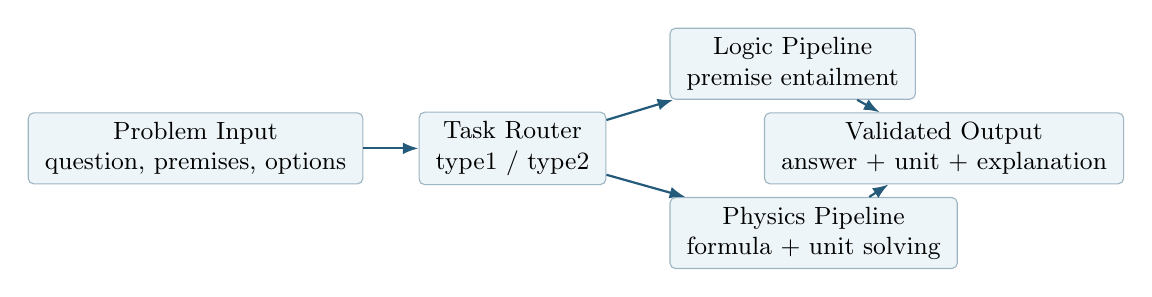
\begin{tikzpicture}[
  node distance=0.5cm and 0.7cm,
  box/.style={draw=line, fill=soft, rounded corners=2pt, align=center,
              minimum height=0.7cm, inner xsep=6pt, font=\small},
  route/.style={draw=accent, -{Latex[length=2mm]}, thick}
]
\node[box] (input) {Problem Input\\question, premises, options};
\node[box, right=of input] (gate) {Task Router\\type1 / type2};
\node[box, above right=0.15cm and 0.8cm of gate] (logic) {Logic Pipeline\\premise entailment};
\node[box, below right=0.15cm and 0.8cm of gate] (phys) {Physics Pipeline\\formula + unit solving};
\node[box, right=2.0cm of gate] (final) {Validated Output\\answer + unit + explanation};
\draw[route] (input) -- (gate);
\draw[route] (gate) -- (logic);
\draw[route] (gate) -- (phys);
\draw[route] (logic) -- (final);
\draw[route] (phys) -- (final);
\end{tikzpicture}
\end{center}

\section*{Shared Cascade: References $\rightarrow$ Judge $\rightarrow$ Reconcile}
Both pipelines use the same three-stage shape. Lightweight reference solvers
produce candidate answers; a single 8B \textbf{judge} solves the problem itself
and then decides; and a \textbf{consensus-reconciliation} step re-checks the
judge whenever the references unanimously disagree with it.
\begin{center}
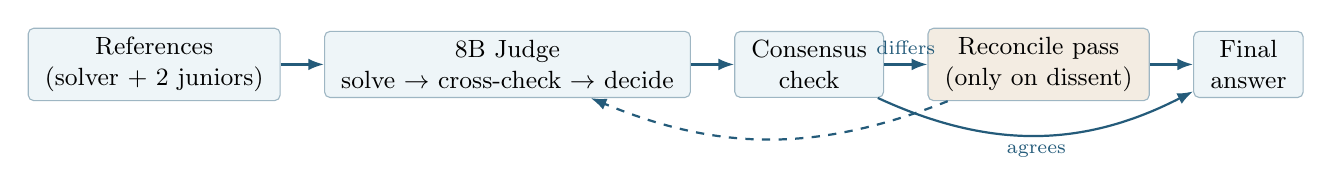
\begin{tikzpicture}[
  node distance=0.45cm and 0.55cm,
  box/.style={draw=line, fill=soft, rounded corners=2pt, align=center,
              minimum height=0.72cm, inner xsep=6pt, font=\small},
  rec/.style={draw=line, fill=warm, rounded corners=2pt, align=center,
              minimum height=0.72cm, inner xsep=6pt, font=\small},
  route/.style={draw=accent, -{Latex[length=2mm]}, thick},
  back/.style={draw=accent, -{Latex[length=2mm]}, thick, dashed}
]
\node[box] (refs) {References\\(solver + 2 juniors)};
\node[box, right=of refs] (judge) {8B Judge\\solve $\rightarrow$ cross-check $\rightarrow$ decide};
\node[box, right=of judge] (check) {Consensus\\check};
\node[rec, right=of check] (recon) {Reconcile pass\\(only on dissent)};
\node[box, right=of recon] (out) {Final\\answer};
\draw[route] (refs) -- (judge);
\draw[route] (judge) -- (check);
\draw[route] (check) -- node[above,font=\scriptsize\color{accent}]{differs} (recon);
\draw[back] (recon) to[bend left=22] (judge);
\draw[route] (recon) -- (out);
\draw[route] (check) to[bend right=26] node[below,font=\scriptsize\color{accent}]{agrees} (out);
\end{tikzpicture}
\end{center}

\section*{Pipeline 1: Logic Questions}
\begin{itemize}
\item \textbf{Purpose:} decide which option (or Yes / No / Not Given) is
logically entailed by the given premises, using ONLY those premises, never
outside knowledge.
\item \textbf{Prompt normalization:} the question becomes a strict examiner
format: numbered premises, optional definitions, the question stem, and options.
\item \textbf{Generator stage:} two independent 4B models solve the same problem
concurrently, each emitting structured JSON with the chosen answer, the premises
it used, and a short explanation.
\item \textbf{Judge stage:} an 8B senior examiner re-derives the answer itself
from the premises and arbitrates between the juniors, guarding against the
classic traps, invalid converse / inverse reasoning, quantifier swaps
(``some'' vs ``all''), and answering ``No'' when only ``Not Given'' is proven.
\item \textbf{Consensus reconciliation:} if both juniors agree on one answer but
the judge contradicts it, the judge gets one extra pass, it must treat the
agreement as strong evidence it slipped, find its own error, and may keep its
dissent only by citing a specific premise that disproves the juniors.
\item \textbf{Finalization:} deterministic code canonicalizes the verdict, maps
it to an exact option, attaches 0-based premise citations, and builds the record.
A weighted-vote mode is also available as an alternative to the judge.
\end{itemize}

\section*{Pipeline 2: Physics Questions}
\begin{itemize}
\item \textbf{Purpose:} compute a numeric or symbolic answer \emph{with the
correct unit}, keeping the reasoning trace explainable.
\item \textbf{Deterministic solver first:} formula and template solvers across
many domains (mechanics, electricity / circuits, thermodynamics, optics, waves
and oscillations, fluids, modern / atomic / nuclear, astrophysics) produce the
first candidate answer, unit, and confidence.
\item \textbf{Two 4B references:} the deterministic answer is given to two 4B
models \emph{as reference only}; each solves the problem independently.
\item \textbf{8B judge (authoritative):} the judge solves from first principles
(stating each vector's direction before combining), cross-checks the three
references, then re-evaluates and decides. Its output is the final answer, the
deterministic and 4B answers are never substituted for it.
\item \textbf{Robust parsing:} a recovery ladder, balanced-JSON parse
$\rightarrow$ tolerant regex $\rightarrow$ a no-think guided-JSON re-extraction of
the judge's own reasoning, guarantees the judge's answer and unit are extracted,
and a unit accidentally placed in the answer field is moved to the unit field
rather than discarded.
\item \textbf{Consensus reconciliation:} if the judge dissents from a unanimous
reference consensus, one extra judge pass forces it to re-derive and locate its
mistake before finalizing.
\item \textbf{Verification:} answer normalization (plain ASCII decimals), ASCII
unit checking, and schema validation prevent malformed numbers or invalid units
from reaching the output.
\end{itemize}

\section*{Shared Infrastructure}
\begin{itemize}
\item \textbf{One resident line-up, swapped on a single GPU:} the two 4B
generators stay co-resident and the 8B judge is woken (generators slept) only for
its judging / reconciliation calls, so at most 8B of weights sit on the GPU at
any moment.
\item \textbf{Structured output:} non-thinking model calls use guided JSON;
thinking calls reason freely and are parsed by the recovery ladder.
\item \textbf{Stub mode:} a deterministic offline backend exercises the full
request / response wiring with no GPU, used by the test suite.
\end{itemize}

\section*{How the Two Pipelines Work Together}
\begin{tabular}{@{}p{0.20\linewidth}p{0.76\linewidth}@{}}
\toprule
\textbf{Step} & \textbf{Pipeline behavior} \\
\midrule
Routing & \texttt{type1} goes to the logic entailment pipeline; \texttt{type2}
goes to the physics solver pipeline; blank types route by shape. \\
Candidate creation & Logic creates two model answers; physics creates a
deterministic solver answer first, then two model-assisted references. \\
Judging & A single 8B judge re-derives the answer from the original problem and
decides, it must not simply copy a candidate. \\
Reconciliation & When the references unanimously disagree with the judge, one
extra judge pass makes it find its own error before committing. \\
Validation & Code enforces the JSON schema, answer normalization, premise
citation, and unit consistency before returning the result. \\
\bottomrule
\end{tabular}

\section*{Key Principle}
\textbf{Use the strongest reasoning method for each task, and never let a single
model overrule a clear consensus on a slip.} Logic questions are solved as
entailment problems with independent generation, judging, and reconciliation.
Physics questions are solved as computations where deterministic solvers and unit
checks anchor the references, an 8B judge owns the final answer, and a recovery
ladder guarantees it is parsed. In both pipelines, deterministic validation turns
the reasoning into a stable, competition-ready output.

\end{document}
